\chapter{Integration}
\section{Methods}
The integration of the system was performed by individually implementing each sub-section
and ensuring that the sub-section's outputs are compatible with adjacent sub-section inputs.

With this methodology in mind, the system was integrated in the order of outputs to inputs.
This is so that with the edition of each new sub-section, the system response to the new sub-section can be verified.

First, the lighting controller was implemented, as shown in the Lighting Controller chapter.
Then, software for the off-body PC was written that could communicate with the lighting controller,
and control the prototyping fixture based on a prerecorded data-set.
The data-set was that of an electrocardiogram sampled at 360 Hz.
The lights were controlled by pulsing their intensity at the peaks of the electrocardiogram.
Then, the software was modified so that the data being processed could be received as a continuous stream, instead of a fixed data-set.

Communication between the on-body device and the off-body PC has already been documented in the On-Body Device chapter.
This communication was expanded upon by receiving the data into the same continuous stream that had already been established with the data-set,
thus allowing the on-body device to control the prototyping fixture through peaks in the transmitted data.

The on-body device needs to collect different types of data with varying sample and transmission rates.
Much like implementing the prototyping fixture for the lighting controller where the end of each DMX frame needed to be marked,
the varying data sizes were implemented using special characters to mark the end of data transmission using base64.
Additionally, packet headers were created to specify the different kinds of data that are being sent
(implementation was prior to the board power distribution issues).


\section{Results}
The off-body PC has a fixed length first-in-first-out buffer that can be filled with either testing data or streamed data from the on-body device.
The received data can control the prototyping fixture, with various methods of control through data processing.
Beat detection was implemented on the testing data-set,
allowing the prototyping fixture to increase intensity at each peak of the input data.

\begin{figure}[!ht]
  \caption{Fixed length FIFO data buffer with testing data-set}\label{fig:matlab_packet_test2}
  \centering
  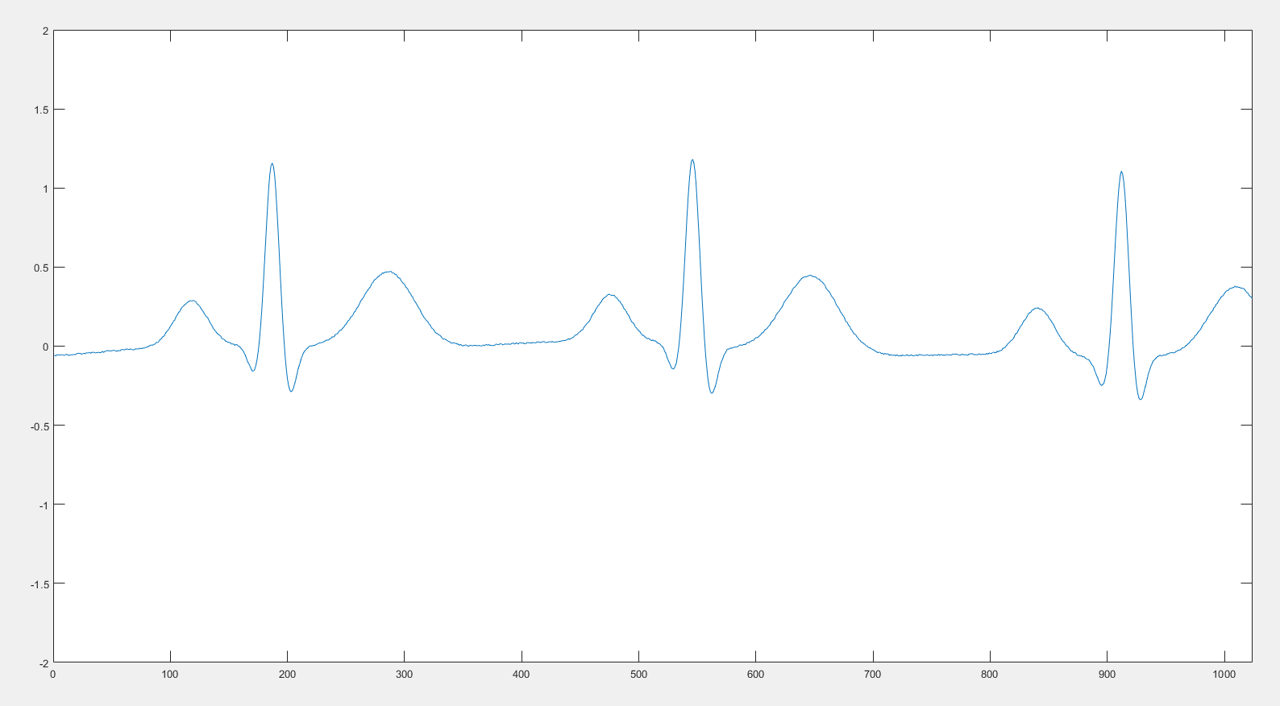
\includegraphics[width=1\columnwidth]{chapters/development/MATLAB/FULL_FILLED}
\end{figure}

The implementation of varying data sizes and the inclusion of packet headers allows data to be effectively transmitted and received.
An unintended benefit of this is that a debug packet header can be specified, and since the data can be variable length,
a fully functional `printf' function on the PIC32 can be used to send arbitrary debugging messages to the off-body PC.

As was presented in the On-Body Device chapter, the PIC32 and ESP32 are able to communicate with the off-body PC at a speed of 1.45 kbits/s.
At a sampling rate of 50 Hz~\cite{Ajdaraga:2017}, the bandwidth is high enough to send 29 bits.
For instance, you could send 8-bits of header information and 16-bits of electrocardiogram data, while maintaining sampling and transmission at 50 Hz.


\section{Discussion}
To reduce the amount of hardware that is required to be worn by the performer,
the bulk of the processing is to be done on an off-body PC.
This PC communicates wirelessly with the on-body device,
receiving sensor data from the various biosignals that the device is measuring.
The PC then must process the data and coordinate the music and lighting generation.

MATLAB was used as the off-body PC language for processing because of ease of use, versatility,
and since it had been previously used on this project.

Since MATLAB functions operate on arrays and matrices,
the desired behaviour of our program is to store a length of data and process it all together,
rather than try to process each sample individually as it arrives.
To keep the system responsive, the buffer is kept at a fixed length,
so that over time the processing does not incrementally take longer due to the increase in data to process.

For testing, an electrocardiogram (ECG) data-set from a previous iteration of the project was used.
The data-set was imported into the workspace in a way that mimicked wireless reception.
Specifically, the data was packetized and shifted into the predefined fixed length buffer.
Then, the program loops, continually sending data as new packets, and repeats once it reaches the end of the data-set.
This is so that processing methods can be developed experimentally
with the assurance that the behaviour will remain consistent once the system transitions away from the testing data-set.

The first processing method that was developed was beats per minute (BPM) prediction using the ECG QRS signal.
This method calculates the BPM of the signal by measuring the gaps between the peaks of the QRS signals.

In order to get these devices to communicate, inbound and outbound rules need to be defined in the off-body PC firewall.
This is to allow connections on the specified port, since most PC ports are typically closed for security reasons.
The port settings can be seen in~\autoref{fig:firewall}.

\begin{figure}[!ht]
  \caption{TCP/IP firewall port settings}\label{fig:firewall}
  \centering
  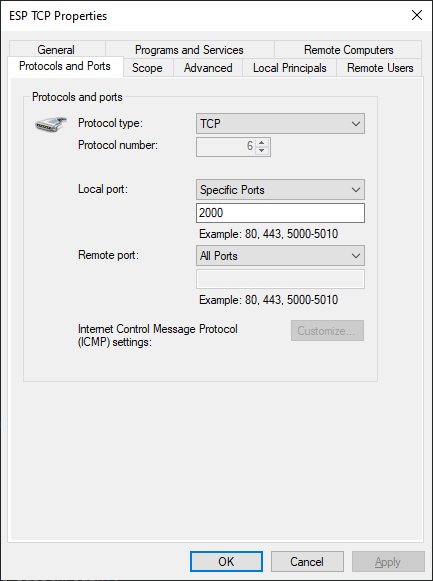
\includegraphics[width=1\columnwidth/2]{chapters/development/FIREWALL}
\end{figure}

The implementation of wireless printf debugging has significant benefits as it not only speeds up debugging
but also allows debugging in the interrupt service routine, which cannot be debugged with breakpoints.
The speed increase of using printf is also seen each time the device is programmed,
as the device takes longer to boot when being put into debugging mode.
Finally, the inclusion of printf debugging allows messages to be sent beyond debugging, such as status, warning, or error messages.
These messages will be received along with the sensor data, potentially giving reason for unexpected behaviour or delays in incoming data.

The speed at which transmission occurs is only fast enough to send a single stream of 24-bit ECG data.
While this may be fine for testing,
the transmission speed will need to increase significantly if this device is ever intended to be used in an actual performance.
As it is likely that a performer would wish to have more than just their heart rate be used to augment the performance.

The final part of the project is the testing and validation.
Unfortunately due to power supply issues, a proper testing and validation suite could not be conducted on the device.
The power issues are related to what was seen earlier with the ESP32.
As more devices came online, the current draw across on-body device's power plane increased, which subsequently increased the voltage drop.
Eventually, this voltage drop became too large and the devices started to lose power.
Thus, the testing and validation of the system remains unfinished, as the device was no longer responsive at the point when testing began.
